\chapter{Empirical Results}
\label{chapter:empirical_results}

\begin{introduction}
\begin{flushright}
``How much money you make?''
\end{flushright}

\vspace{0.5em}

This chapter presents the out-of-sample evaluation of all developed frameworks, feature variants, and benchmark strategies on the held-out test period. Results are reported through standard portfolio performance metrics and complemented by cumulative return curves and weight allocation dynamics, organized by framework and variant.
\end{introduction}


As outlined in Chapter~\ref{chapter:methods}, all results presented in this chapter are based on a held-out test set spanning the final two years of the dataset, from July 1, 2023 to June 30, 2025. This approach ensures that each model is evaluated on data not seen during training, thereby providing a robust assessment of its generalization capability. Additionally, a mid-period refit is conducted one year into the evaluation window, on July 1, 2024. This refit allows the models to update their parameters and adapt to any structural changes in the market dynamics that may have occurred, thereby enhancing their performance in the second year.

The results are organized by approach and variant, covering the features selected during hyperparameter search, the portfolio-level performance metrics, and visualizations of both cumulative returns and weight dynamics.

The primary performance metrics employed in this study are those most used in the empirical portfolio optimization literature. These include cumulative return, annualized volatility, maximum drawdown, and risk-adjusted return measures. Together, these metrics provide a comprehensive assessment of both the return-generating ability and the downside risk profile of each strategy, as summarized in Table~\ref{tab:portfolio_optimization_metrics}.

The risk-adjusted performance measure, namely Sharpe ratio, requires the specification of a risk-free rate. While the choice of risk-free rate may vary across studies, this work follows the standard convention in the asset pricing literature, as in Fama and French \cite{e60f7}, by using the 1-month U.S.\ Treasury Bill yield. This proxy is widely adopted and is obtained from the Federal Reserve Economic Data (FRED) database\footnote{\url{https://fred.stlouisfed.org/series/DGS1MO}}.

\section{Benchmarks}

Two benchmark strategies are evaluated to provide a performance baseline to be compared against. The first is a naive equal-weight (EW) portfolio serving as a parameter-free reference, and the second is a mean-variance optimized portfolio using CAPM-implied expected returns (MVO--CAPM), representing a classical quantitative approach.

\subsection{Equal-Weighted Portfolio: EW}

The EW strategy provides the most conservative reference point, allocating capital uniformly across all 11 sector ETFs and rebalancing daily to maintain equal exposure regardless of tradable assets. Over the two-year test period, the strategy achieves a cumulative return of 1.315, annualized volatility of 0.137, a Sharpe ratio of 0.704, and a maximum drawdown of $-$0.153 (Table~\ref{tab:ew_metrics}).

\begin{table}[ht]
\centering
\caption{Out-of-sample performance metrics for EW benchmark, including cumulative return, volatility, Sharpe ratio, and maximum drawdown.}
\label{tab:ew_metrics}
\renewcommand{\arraystretch}{1.2}
\begin{tabular}{|c|c|c|c|c|}
\hline
\textbf{Variant} & \textbf{Cum.\ Return} & \textbf{Volatility} & \textbf{Sharpe Ratio} & \textbf{Max Drawdown} \\
\hline
Benchmark & $1.315$ & $0.137$ & $0.704$ & $-0.153$ \\
\hline
\end{tabular}
\end{table}

\begin{figure}[ht]
    \centering
    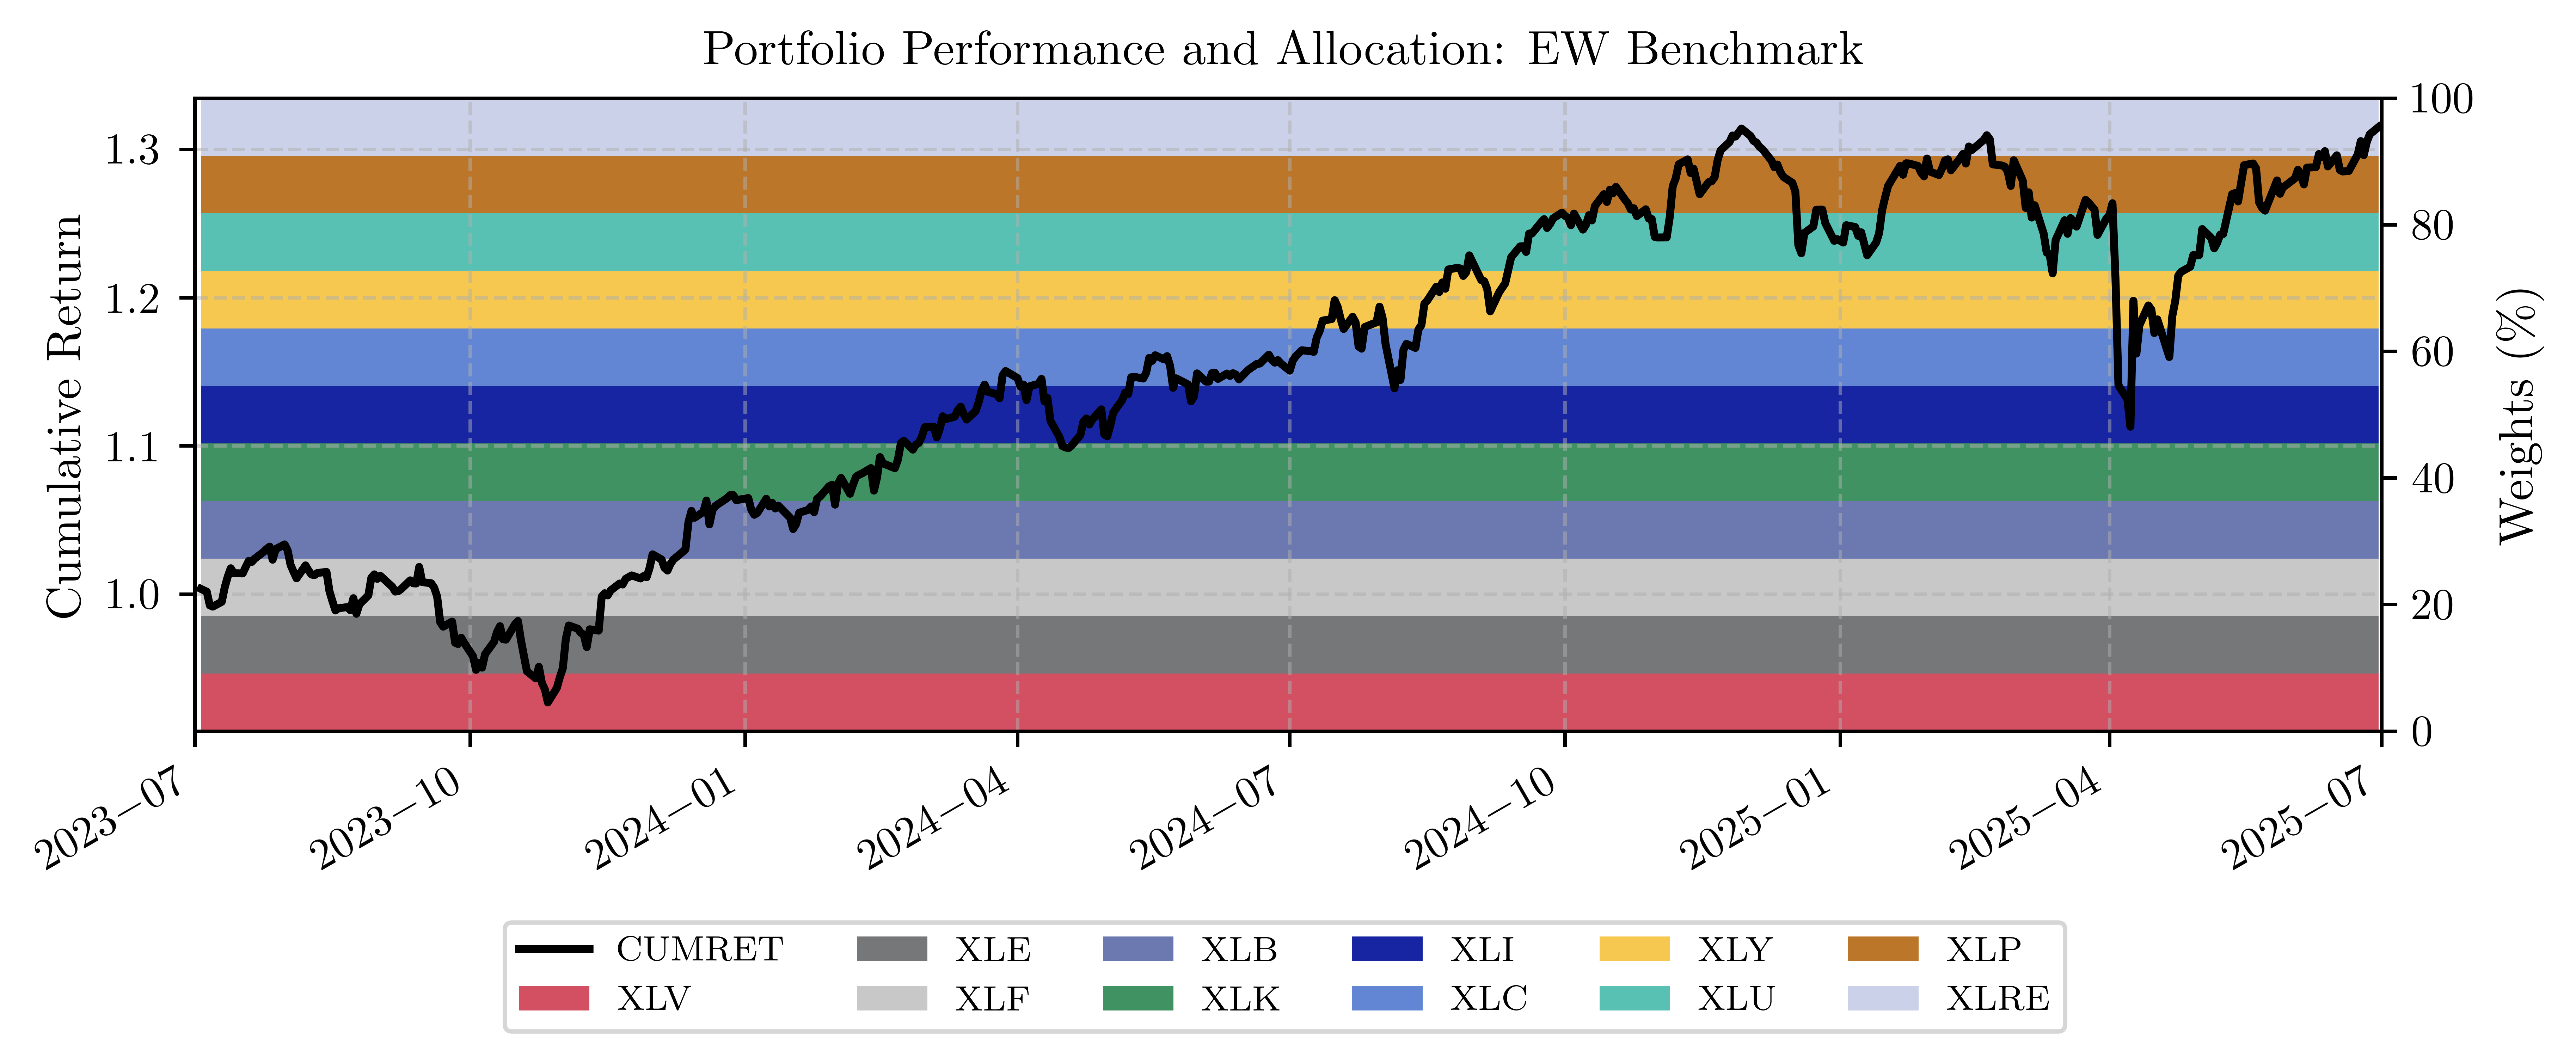
\includegraphics[width=1\textwidth]{figs/CUMRET_WEIGHTS_EW.png}
    \caption{Cumulative portfolio returns (black line) alongside sector ETF allocation weights (stacked areas) over the test period for the EW benchmark.}
    \label{fig:cumret_weights_ew}
\end{figure}

Fig.~\ref{fig:cumret_weights_ew} presents the portfolio's cumulative return (left axis) alongside the daily sector weight decomposition (right axis) across the full evaluation window. The cumulative return begins at 1.00 (100\% of initial capital), rises to approximately 1.25 by October 2024, followed by a brief pause and a modest drawdown, and ends the test period at approximately 1.32 (a 32\% gain over the initial capital). Because the equal-weight constraint fixes each sector at $1/11 \approx 9.1\%$ (since the tradable assets are 11 ETFs), the weight panel shows 11 uniformly thick horizontal bands throughout the entire two-year window.


\subsection{Mean-Variance Optimisation with CAPM Priors: MVO--CAPM}

The MVO--CAPM benchmark introduces an explicit optimization step: CAPM-implied expected returns are computed from historical betas against the S\&P~500 and fed into a mean-variance optimizer that maximizes the portfolio Sharpe ratio subject to long-only constraints. Ridge regularization stabilizes the covariance matrix, and all hyperparameters (including the rebalance frequency) are tuned. As reported in Table~\ref{tab:mvo_capm_metrics}, this approach improves on the EW baseline in terms of cumulative return (1.380) and Sharpe ratio (0.835), but does so at the cost of higher volatility (0.146) and a wider maximum drawdown ($-$0.188), indicating that the improvement in risk-adjusted return is driven by higher absolute returns rather than by improved downside-risk control.

\begin{table}[ht]
\centering
\caption{Out-of-sample performance metrics for MVO--CAPM benchmark, including cumulative return, volatility, Sharpe ratio, and maximum drawdown.}
\label{tab:mvo_capm_metrics}
\renewcommand{\arraystretch}{1.2}
\begin{tabular}{|c|c|c|c|c|}
\hline
\textbf{Variant} & \textbf{Cum.\ Return} & \textbf{Volatility} & \textbf{Sharpe Ratio} & \textbf{Max Drawdown} \\
\hline
Benchmark & $1.380$ & $0.146$ & $0.835$ & $-0.188$ \\
\hline
\end{tabular}
\end{table}

\begin{figure}[ht]
    \centering
    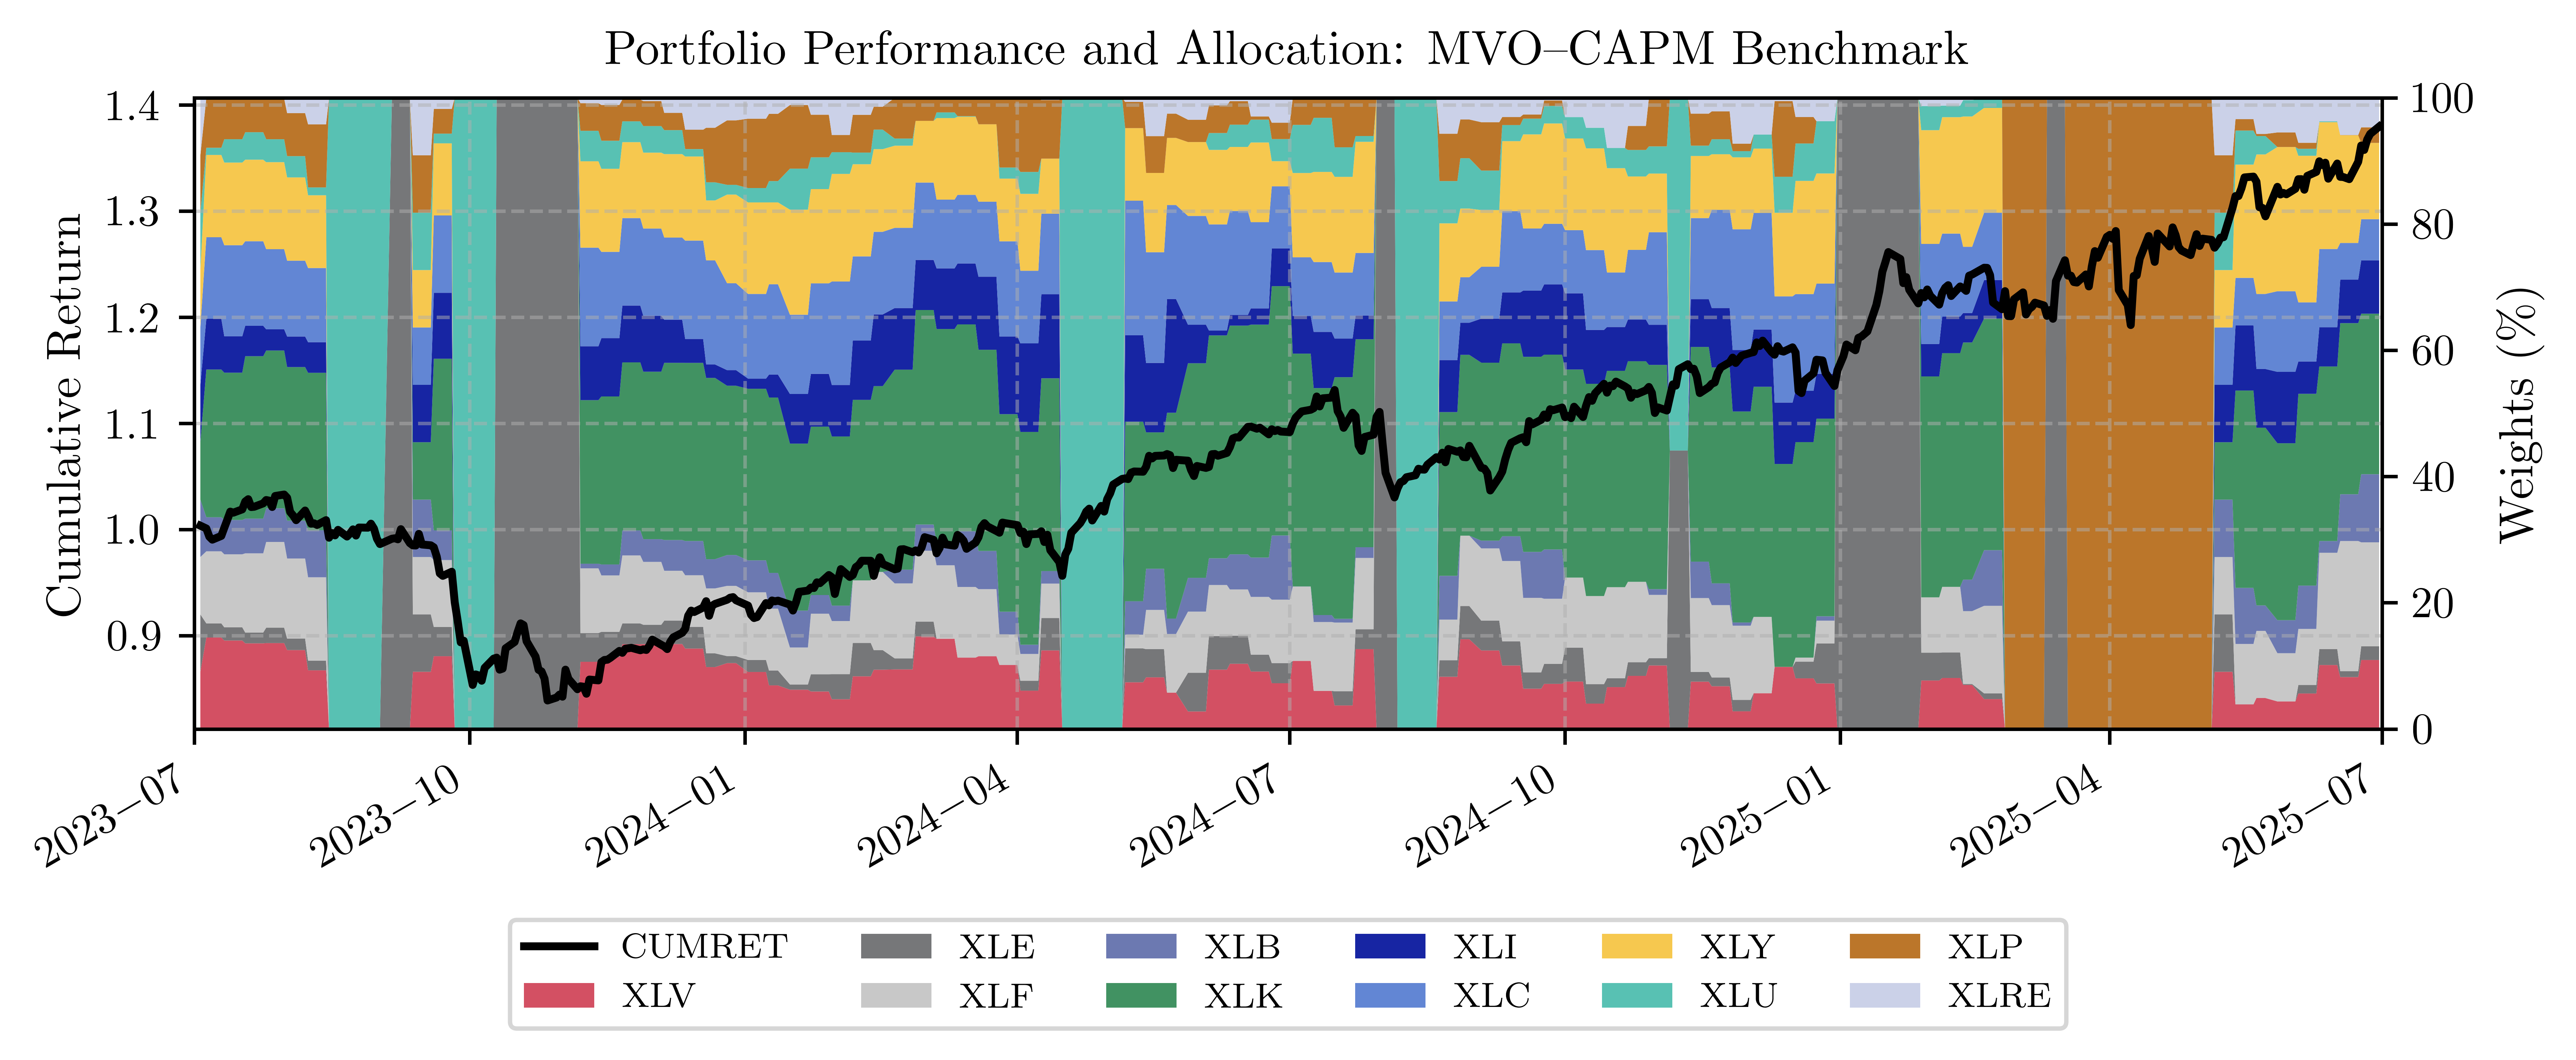
\includegraphics[width=1\textwidth]{figs/CUMRET_WEIGHTS_MVO-CAPM.png}
    \caption{Cumulative portfolio returns (black line) alongside sector ETF allocation weights (stacked areas) over the test period for the MVO--CAPM benchmark.}
    \label{fig:cumret_weights_mvo_capm}
\end{figure}

Fig.~\ref{fig:cumret_weights_mvo_capm} illustrates the behavior of the MVO--CAPM benchmark, showing cumulative returns and sector weight dynamics over the test period. The MVO--CAPM cumulative return curve follows a more irregular trajectory than that of the EW strategy (Fig.~\ref{fig:cumret_weights_ew}), with a steadier ascent after a visible drawdown in mid-to-late 2023. Unlike the uniform bands of the EW strategy, the weight panel shows substantial time-variation: XLK (Information Technology) receives a larger allocation for most of the period, while other sectors, such as XLU (Utilities), XLE (Energy), and XLP (Consumer Staples), receive near-100\% allocations at certain points. For instance, in August 2024, XLU (Utilities) receives a near-complete allocation, which is associated with a drawdown relative to the EW strategy, and conversely, in April 2025, XLP (Consumer Staples) receives a near-100\% allocation, allowing the strategy to avoid a drawdown observed in the EW benchmark.


\section{Reinforcement Learning Agent: DRL--PPO}

The DRL--PPO agent learns a portfolio allocation policy by interacting with the market environment and maximizing the Differential Sharpe Ratio reward. Four variants are evaluated, each involving a different set of input features, as described previously.

The hyperparameter search selected the feature configuration shown in Table~\ref{tab:drlppo_features}. The technical feature set comprises the closing price, the long-term moving average (\texttt{252d\_SMA}), RSI, volume, and five-day volatility, together with VIX. GDELT sentiment features are admitted at a confidence threshold of 0.75 and focus on count-based sentiment indicators and short-horizon variations of balance ratio, reflecting the agent's tendency to exploit sharp sentiment shifts rather than level estimates. Reddit sentiment uses the same threshold and selects balance-ratio levels and their lagged values, capturing the persistence of sector-specific investor mood across previous trading sessions.

\begin{table}[ht]
\centering
\caption{DRL--PPO framework selected features for each variant (Technical, GDELT, and Reddit).}
\label{tab:drlppo_features}
\renewcommand{\arraystretch}{1.2}
\begin{tabular}{|cc|c|c|}
\hline
\multicolumn{2}{|c|}{\textbf{Technical}} & \textbf{GDELT} & \textbf{Reddit} \\
\hline
\multicolumn{2}{|c|}{--} & Threshold: 0.75 & Threshold: 0.75 \\
\hline
\texttt{Close}      & \texttt{5d\_Vol}      & \texttt{countPos} & \texttt{balance\_ratio} \\
\texttt{252d\_SMA}  & \texttt{VIX\_Close}   & \texttt{countNeg} & \texttt{BR\_Lag1} \\
\texttt{RSI}        & --                    & \texttt{BR\_Var1} & \texttt{BR\_Lag5} \\
\texttt{Volume}     & --                    & \texttt{BR\_Var5} & -- \\
\hline
\end{tabular}
\end{table}

Table~\ref{tab:drlppo_metrics} shows that the Technical variant achieves performance close to the stronger benchmark (MVO--CAPM) in terms of Sharpe ratio (0.809 vs.\ 0.835), suggesting that the agent is able to learn an effective allocation policy from price- and volume-based features alone.

Adding GDELT-based sentiment produces a clear improvement (Sharpe ratio: 0.976) and notably reduces both volatility (from 0.147 to 0.140) and maximum drawdown (from $-$0.152 to $-$0.116), suggesting that GDELT-derived signals act as a stabilizing input to the policy rather than an aggressive directional signal. Adding Reddit-based sentiment produces the largest single-source improvement among all DRL--PPO variants: cumulative return rises from 1.371 to 1.538 and the Sharpe ratio reaches 1.173. The combined GDELT+Reddit variant achieves the highest Sharpe ratio (1.222) and cumulative return (1.596) across all DRL--PPO configurations.

\begin{table}[ht]
\centering
\caption{Out-of-sample performance metrics for DRL--PPO framework variants, including cumulative return, volatility, Sharpe ratio, and maximum drawdown.}
\label{tab:drlppo_metrics}
\renewcommand{\arraystretch}{1.2}
\begin{tabular}{|c|c|c|c|c|}
\hline
\textbf{Variant} & \textbf{Cum.\ Return} & \textbf{Volatility} & \textbf{Sharpe Ratio} & \textbf{Max Drawdown} \\
\hline
Technical       & $1.371$ & $0.147$ & $0.809$ & $-0.152$ \\
\hline
GDELT           & $1.424$ & $0.140$ & $0.976$ & $-0.116$ \\
\hline
Reddit          & $1.538$ & $0.151$ & $1.173$ & $-0.147$ \\
\hline
GDELT+Reddit    & $1.596$ & $0.162$ & $1.222$ & $-0.130$ \\
\hline
\end{tabular}
\end{table}

\begin{figure}[H]
    \centering
    \includegraphics[width=1\textwidth]{figs/CUMRET_WEIGHTS_DRLPPO.png}
    \caption{Cumulative portfolio returns (black line) alongside sector ETF allocation weights (stacked areas) over the test period for each variant within the DRL--PPO framework.}
    \label{fig:cumret_weights_drlppo}
\end{figure}

Fig.~\ref{fig:cumret_weights_drlppo} displays the cumulative return curves and portfolio weight decompositions for the four DRL--PPO variants (Technical, GDELT, Reddit, and GDELT+Reddit, respectively).

Unlike the benchmarks, all DRL--PPO variants show a notable regime change at the refit point (July 1, 2024), where the sector allocations shift markedly. The Technical variant shows highly variable weights in the first year, with a focus on XLE (Energy), transitioning to a more stable allocation in the second year. The GDELT variant exhibits more stable weights across both years, with the dominant allocation shifting from XLY (Consumer Discretionary) and XLK (Information Technology) in the first year to XLV (Health Care) and XLU (Utilities) in the second. The Reddit variant shows a clear shift at the refit point: the first year is characterized by short-term bets concentrated on XLP (Consumer Staples) and XLK (Information Technology), while the second year shows a more stable focus on XLK (Information Technology). Finally, the GDELT+Reddit variant also shows a clear regime change at the refit point, with both periods characterized by rapid short-term weight variation, primarily in XLK (Information Technology), and a greater focus on XLP (Consumer Staples) and XLU (Utilities) in the second year. Most notably, larger weight shifts appear around November 2023, January 2025, and April 2025, coinciding with sharper movements in the cumulative return curve, suggesting that the agent is able to adapt quickly to changing market conditions by adjusting its sector allocations in response to new information.


\section{Predict-Then-Optimize: LSTM--BL}

This two-stage approach first trains an ensemble of LSTM models to predict next-day sector returns. Cross-model disagreement is used to quantify view uncertainty. The resulting predictions and their associated uncertainty are then fed into a Black-Litterman optimizer, which blends them with an equal-weight equilibrium prior, yielding portfolio weights that become more aggressive when the ensemble is confident and more conservative when it disagrees. Ensemble membership is determined by the Spearman Information Coefficient (IC) across walk-forward folds, and the top $N$ configurations are retained. In this case, $N$ was set to 3 by the Black-Litterman tuning process, as $N$ was included as a hyperparameter.

Table~\ref{tab:lstmvreturns_features} presents the selected features for each ensemble member.
All three members rely on an identical set of technical inputs: OHLC prices, 63-day moving average, RSI, volume, and VIX closing price. The only difference is that Rank 2 selects five-day volatility instead of Bollinger Bands, suggesting that the technical signals with the highest predictive power for returns are consistent across different model configurations. In contrast, GDELT and Reddit feature selections vary more across ensemble members, including the choice of confidence thresholds. Rank 1 applies a moderate confidence threshold for both GDELT (0.50) and Reddit (0.75), Rank 2 loosens the GDELT threshold to 0.00 (admitting all labelled items) while keeping Reddit at 0.75, and Rank 3 applies the most restrictive threshold (0.90) for both sources. This variation suggests that different ensemble members capture different aspects of the sentiment signal, with some prioritizing breadth (Rank 2) and others prioritizing label quality (Rank 3).

\begin{table}[ht]
\centering
\caption{LSTM--BL framework selected features for each variant (Technical, GDELT, and Reddit), for the returns prediction stage.}
\label{tab:lstmvreturns_features}
\renewcommand{\arraystretch}{1.2}
\begin{tabular}{|cc|c|c|}
\hline
\multicolumn{2}{|c|}{\textbf{Technical}} & \textbf{GDELT} & \textbf{Reddit} \\
\hline\hline
\multicolumn{4}{|l|}{\textit{Rank 1}} \\
\hline
\multicolumn{2}{|c|}{--} & Threshold: 0.50 & Threshold: 0.75 \\
\hline
\texttt{Close}  & \texttt{RSI}          & \texttt{balance\_ratio} & \texttt{balance} \\
\texttt{Open}   & \texttt{Volume}       & \texttt{BR\_Rolling22} & -- \\
\texttt{High}   & \texttt{BBUpper}      & -- & -- \\
\texttt{Low}    & \texttt{BBLower}      & -- & -- \\
\texttt{63d\_SMA}  & \texttt{VIX\_Close} & -- & -- \\
\hline\hline
\multicolumn{4}{|l|}{\textit{Rank 2}} \\
\hline
\multicolumn{2}{|c|}{--} & Threshold: 0.00 & Threshold: 0.75 \\
\hline
\texttt{Close} & \texttt{RSI} & \texttt{balance\_ratio} & \texttt{balance\_ratio} \\
\texttt{Open} & \texttt{Volume} & \texttt{BR\_Rolling3} & -- \\
\texttt{High} & \texttt{5d\_Vol} & -- & -- \\
\texttt{Low} & \texttt{VIX\_Close} & -- & -- \\
\texttt{63d\_SMA} & -- & -- & -- \\
\hline\hline
\multicolumn{4}{|l|}{\textit{Rank 3}} \\
\hline
\multicolumn{2}{|c|}{--} & Threshold: 0.90 & Threshold: 0.90 \\
\hline
\texttt{Close} & \texttt{RSI} & \texttt{balance} & \texttt{countPos} \\
\texttt{Open} & \texttt{Volume} & \texttt{BR\_Rolling3} & \texttt{countNeg} \\
\texttt{High} & \texttt{BBUpper} & -- & \texttt{BR\_Var1} \\
\texttt{Low} & \texttt{BBLower} & -- & \texttt{BR\_Var5} \\
\texttt{63d\_SMA} & \texttt{VIX\_Close} & -- & -- \\
\hline
\end{tabular}
\end{table}

Fig.~\ref{fig:returns_metrics_results_violin} and Table~\ref{tab:lstmvreturns_metrics_returns} present the ensemble's forecasting performance across the four variants. The figure shows the distribution of error metrics (MSE, RMSE, MAPE) by sector and variant, providing a cross-sectional view of forecast accuracy, while the table summarizes the mean values of these metrics alongside the predictive Spearman IC and Rank IC.

\begin{figure}[ht]
    \centering
    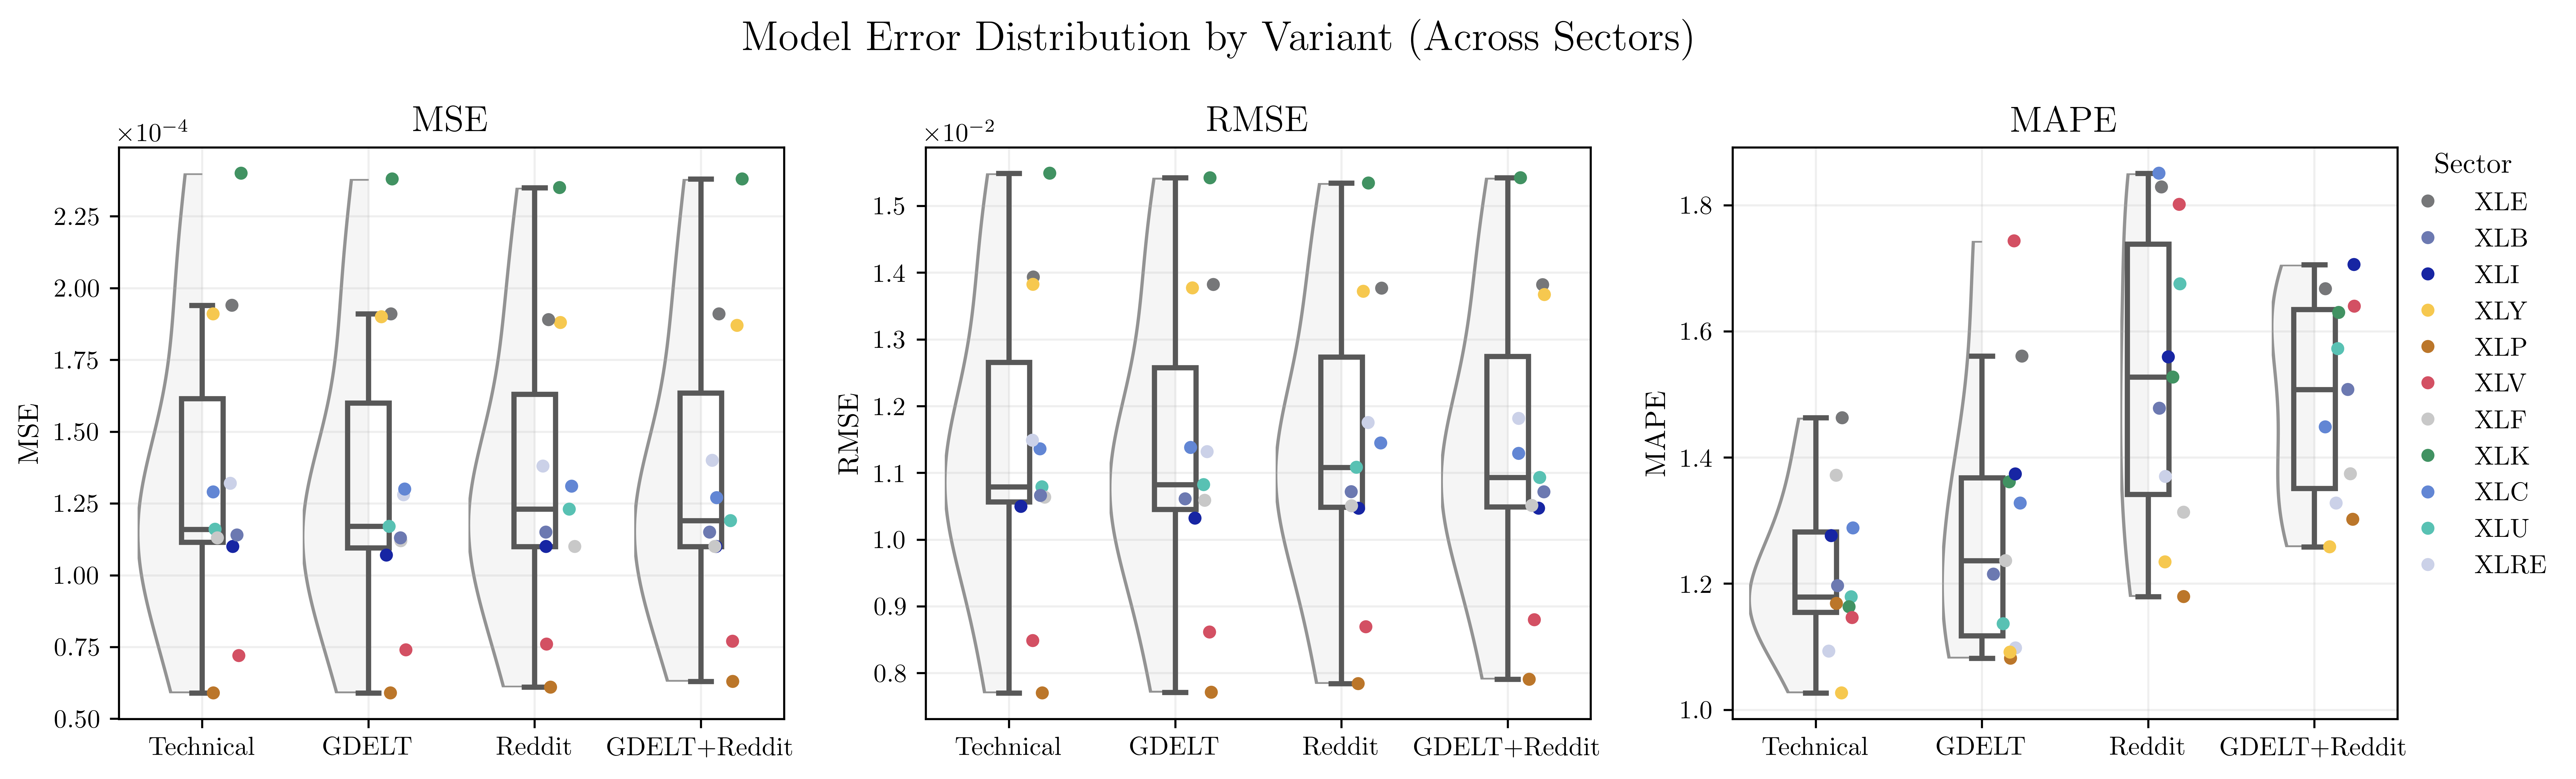
\includegraphics[width=1\textwidth]{figs/returns_metrics_violin.png}
    \caption{Error distributions (MSE, RMSE, and MAPE) for ensemble return prediction models across different variants. Violin plots depict full distributional shape, boxplots summarize central tendency and spread, and points represent sector-level ETF observations.}
    \label{fig:returns_metrics_results_violin}
\end{figure}

\begin{table}[ht]
\centering
\caption{Out-of-sample performance of LSTM return prediction ensembles under each variant. Metrics include error-based measures (MSE, RMSE, MAPE) and correlation-based measures of predictive signal quality (Spearman IC and Rank IC).}
\label{tab:lstmvreturns_metrics_returns}
\renewcommand{\arraystretch}{1.2}
\begin{tabular}{|c|c|c|c|c|c|}
\hline
\textbf{Variant} & \textbf{MSE} & \textbf{RMSE} & \textbf{MAPE} & \textbf{IC} & \textbf{Rank IC} \\
\hline
Technical & $0.000134$ & $0.011351$ & $1.215700$ & $0.025616$ & $0.331055$ \\
\hline
GDELT & $0.000133$ & $0.011307$ & $1.293273$ & $0.009388$ & $0.014119$ \\
\hline
Reddit & $0.000134$ & $0.011394$ & $1.528918$ & $0.008727$ & $0.008807$ \\
\hline
GDELT+Reddit & $0.000134$ & $0.011395$ & $1.494008$ & $0.019645$ & $0.033853$ \\
\hline
\end{tabular}
\end{table}

The Technical variant consistently achieves median errors equal to or lower than those of the sentiment-augmented variants, suggesting that price and volume variables are sufficient to capture most of the predictive signal in the returns of the analyzed ETFs. The MSE and RMSE distributions are largely overlapping across all four variants, with narrow interquartile ranges and nearly coincident medians. The MAPE distributions show a wider spread, as expected given its percentage-based units, and adding GDELT or Reddit features does not translate into a systematic reduction in relative error: it is associated with greater dispersion across sectors. At the sector level, XLP (Consumer Staples) consistently shows lower errors across all variants, likely owing to its more stable return profile, while more volatile sectors such as XLE (Energy) exhibit higher errors.

Despite the lower Spearman IC under sentiment augmentation, reflected in the ensemble presented results, downstream portfolio performance diverges substantially from the forecasting metrics. As shown in Table~\ref{tab:lstmvreturns_metrics_portfolio}, the Technical variant delivers the weakest performance, with the lowest Sharpe ratio (0.765) and cumulative return (1.347) among all configurations. Introducing GDELT-based sentiment partially reverses this outcome, yielding a modest improvement as the Sharpe ratio increases to 0.817. In parallel, incorporating Reddit sentiment produces the most pronounced single-source gains among all LSTM--BL variants, raising cumulative returns to 1.481, increasing the Sharpe ratio to 1.164, reducing volatility to 0.134, and improving maximum drawdown to $-$0.097. Finally, the combined GDELT+Reddit variant achieves a Sharpe ratio of 0.967, also outperforming the Technical variant.

\begin{table}[ht]
\centering
\caption{Out-of-sample performance metrics for LSTM--BL framework variants, including cumulative return, volatility, Sharpe ratio, and maximum drawdown.}
\label{tab:lstmvreturns_metrics_portfolio}
\renewcommand{\arraystretch}{1.2}
\begin{tabular}{|c|c|c|c|c|}
\hline
\textbf{Variant} & \textbf{Cum.\ Return} & \textbf{Volatility} & \textbf{Sharpe Ratio} & \textbf{Max Drawdown} \\
\hline
Technical & $1.347$ & $0.143$ & $0.765$ & $-0.149$ \\
\hline
GDELT & $1.360$ & $0.139$ & $0.817$ & $-0.159$ \\
\hline
Reddit & $1.481$ & $0.134$ & $1.164$ & $-0.097$ \\
\hline
GDELT+Reddit & $1.416$ & $0.138$ & $0.967$ & $-0.117$ \\
\hline
\end{tabular}
\end{table}

The divergence between forecasting accuracy and portfolio performance can be understood through the nature of the Black-Litterman framework. In this implementation, the view uncertainty matrix $\Omega$ is derived from the dispersion across ensemble members, meaning that a variant whose models disagree more will automatically receive wider confidence intervals on its views, causing the optimizer to fall back more heavily toward the equilibrium prior. This self-regulating mechanism means that noisier forecasts do not translate linearly into worse portfolio weights: the Black-Litterman framework partially absorbs and discounts uncertainty rather than acting on it blindly. Additionally, portfolio performance is jointly determined by the covariance structure of assets, the equilibrium prior, and the interaction between views and the risk-aversion parameter, all of which are independent of forecast accuracy. These considerations also suggest that optimizing model selection purely on forecasting metrics such as IC may not align with the downstream objective of portfolio performance within a Black-Litterman framework.

Fig.~\ref{fig:cumret_weights_lstmvreturns} displays the cumulative return curves and weight decompositions for the four LSTM--BL variants (Technical, GDELT, Reddit, and GDELT+Reddit, respectively).

None of the variants show a clear regime change at the refit point (July 1, 2024), with all sectors traded throughout the full evaluation window. The weight panels show frequent short-term allocation shifts across different sectors, with no sustained concentration in any single sector. Beyond the cumulative return curve itself, the weight dynamics do not lend themselves to a straightforward visual interpretation.

% imagem inserted in the section above (fig:cumret_weights_lstmvreturns)


\section{End-to-End Optimization: LSTM--SR}

This framework trains a shared LSTM encoder and a cross-asset Transformer mixer end-to-end by directly maximizing the portfolio Sharpe ratio, eliminating any intermediate return-forecasting step. The architecture outputs portfolio weights directly, with gradients flowing from the Sharpe ratio objective back through the full network.

The selected feature configuration (Table~\ref{tab:lstmvsharpe_features}) incorporates full OHLC price data alongside directional indicators (ADX, CCI), percentage volume change, and Bollinger Bands for volatility context. GDELT sentiment is admitted at a high confidence threshold of 0.90, meaning only items classified with at least 90\% certainty contribute to the feature set, limiting volume but improving label quality. The selected news features focus on aggregate sentiment balance and its short-horizon rate of change. Reddit sentiment operates at a lower threshold of 0.50, allowing a broader range of items, and selects only the aggregate balance ratio without historical variants.

\begin{table}[ht]
\centering
\caption{LSTM--SR framework selected features for each variant (Technical, GDELT, and Reddit).}
\label{tab:lstmvsharpe_features}
\renewcommand{\arraystretch}{1.2}
\begin{tabular}{|cc|c|c|}
\hline
\multicolumn{2}{|c|}{\textbf{Technical}} & \textbf{GDELT} & \textbf{Reddit} \\
\hline
\multicolumn{2}{|c|}{--} & Threshold: 0.90 & Threshold: 0.50 \\
\hline
\texttt{Close} & \texttt{CCI} & \texttt{balance} & \texttt{balance\_ratio} \\
\texttt{Open} & \texttt{Volume\_PctChange} & \texttt{BR\_Var1} & -- \\
\texttt{High} & \texttt{BBUpper} & \texttt{BR\_Var5} & -- \\
\texttt{Low} & \texttt{BBLower} & -- & -- \\
\texttt{ADX} & -- & -- & -- \\
\hline
\end{tabular}
\end{table}

% image belongs to the section above (LSTM--BL)
\begin{figure}[H]
    \centering
    \includegraphics[width=1\textwidth]{figs/CUMRET_WEIGHTS_LSTMvreturns.png}
    \caption{Cumulative portfolio returns (black line) alongside sector ETF allocation weights (stacked areas) over the test period for each variant within the LSTM--BL framework.}
    \label{fig:cumret_weights_lstmvreturns}
\end{figure}

As shown in Table~\ref{tab:lstmvsharpe_metrics}, the Technical variant delivers performance comparable to the stronger benchmark (MVO--CAPM).

The addition of GDELT-based sentiment produces a clear improvement, with the Sharpe ratio rising from 0.829 to 0.907, while also reducing volatility from 0.197 to 0.164 and improving maximum drawdown from $-$0.238 to $-$0.149, suggesting that GDELT-derived signals act as a stabilizing input to the policy rather than an aggressive directional signal. Reddit-based sentiment produces a dramatic improvement against the Technical variant, with the the cumulative return rising from 1.471 to 1.855, nearly doubling the gain over the initial capital (from 47.1\% to 85.5\%), and the Sharpe ratio rises from 0.829 to 1.212. However, this performance comes with a higher volatility (0.238) and a larger maximum drawdown ($-$0.257), indicating that the end-to-end objective amplifies the directional bets suggested by Reddit signals without self-imposed risk constraints. The combined GDELT+Reddit variant achieves a balanced outcome, positioned between the two single-source configurations: a strong Sharpe ratio of 1.081 with volatility and drawdown at more moderate levels than the Reddit-only variant.

\begin{table}[ht]
\centering
\caption{Out-of-sample performance metrics for LSTM--SR framework variants, including cumulative return, volatility, Sharpe ratio, and maximum drawdown.}
\label{tab:lstmvsharpe_metrics}
\renewcommand{\arraystretch}{1.2}
\begin{tabular}{|c|c|c|c|c|}
\hline
\textbf{Variant} & \textbf{Cum.\ Return} & \textbf{Volatility} & \textbf{Sharpe Ratio} & \textbf{Max Drawdown} \\
\hline
Technical & $1.471$ & $0.197$ & $0.829$ & $-0.238$ \\
\hline
GDELT & $1.447$ & $0.164$ & $0.907$ & $-0.149$ \\
\hline
Reddit & $1.855$ & $0.238$ & $1.212$ & $-0.257$ \\
\hline
GDELT+Reddit & $1.580$ & $0.181$ & $1.081$ & $-0.161$ \\
\hline
\end{tabular}
\end{table}

Fig.~\ref{fig:cumret_weights_lstmvsharpe} displays the cumulative return curves and weight decompositions for the four LSTM--SR variants (Technical, GDELT, Reddit, and GDELT+Reddit, respectively).

For the Technical variant, the refit point is not clearly noticeable in the weight dynamics: assets are traded actively with no sustained focus on any single sector and considerable short-term weight variation. However, it is possible to identify that some sectors are barely traded, such as XLB (Materials), XLF (Financials), and XLY (Consumer Discretionary). The April 2024 drawdown also shows a longer recovery duration compared with the other variants in this framework.

The GDELT variant shows no discernible change at the refit point, with all sectors actively traded throughout the evaluation window. Larger weight shifts appear to coincide with sharper movements in the cumulative return curve, suggesting that the model adapts quickly to changing market conditions. XLK (Information Technology) appears to carry the largest weight for most of the period.

The Reddit variant shows a markedly concentrated behavior, allocating almost exclusively to XLK (Information Technology) for the entire two-year window, with XLP (Consumer Staples) receiving some allocation in the second year during periods of higher volatility in the cumulative return curve. Although this variant achieves the highest Sharpe ratio in the approach (1.212), the extreme concentration implies significant exposure to sector-specific risk, which is consistent with the higher volatility and maximum drawdown observed.

%Finally, the GDELT+Reddit variant shows a clear regime change at the refit point: the first year is dominated by an almost exclusive allocation to XLK (Information Technology) (closely resembling the Reddit variant strategy), while the second-year transitions to a more diversified allocation across all sectors, more closely resembling the GDELT variant strategy. This shift aligns with the performance metrics, which reflect a blend of the characteristics of the two single-source variants.
Finally, the GDELT+Reddit variant shows a clear regime change at the refit point: the first year is dominated by an almost exclusive allocation to XLK (Information Technology) (closely resembling the Reddit variant strategy), while the second-year transitions to a more diversified allocation across all sectors (closely resembling the GDELT variant strategy). One possible interpretation is that the first year was characterized by stronger Reddit sentiment signals, and that following the refit and a potential shift in market dynamics, the model identified more stable patterns in GDELT sentiment, prompting the transition to a more diversified allocation in the second year.

\begin{figure}[ht]
    \centering
    \includegraphics[width=1\textwidth]{figs/CUMRET_WEIGHTS_LSTMvsharpe.png}
    \caption{Cumulative portfolio returns (black line) alongside sector ETF allocation weights (stacked areas) over the test period for each variant within the LSTM--SR framework.}
    \label{fig:cumret_weights_lstmvsharpe}
\end{figure}